	\documentclass[10pt,handout]{beamer}
	
	\usetheme{Berlin}
	\usecolortheme{beaver}
	%\usefonttheme[onl]{name}
	
	
	
	\usepackage[utf8]{inputenc} 
	\usepackage[T1]{fontenc} 
	\usepackage{amsmath,amsfonts,pdfsync,color,graphicx}
	\usepackage{amssymb,amsthm,latexsym}
	\usepackage{epstopdf}						
	\usepackage[spanish]{babel}			
	\usepackage{tikz-cd} 					
	\usepackage{setspace} 					
	\usepackage{color}						
	\usepackage{multicol}
	\usepackage{lmodern}
	\usepackage[export]{adjustbox}
	
	
	\usepackage{tikz}
	\tikzset{
		every overlay node/.style={
			draw=white,
			anchor=north west,
		},
	}
	\def\tikzoverlay{%
		\tikz[baseline,overlay]\node[every overlay node]
	}
	
	\DeclareMathOperator{\minim}{min}
	\DeclareMathOperator{\maxim}{max}
	
	\definecolor{grey}{rgb}{0.21, 0.27, 0.31}
	\definecolor{reddy}{rgb}{0.65, 0.11, 0.11}
	
	\title{Home Depot}
	\author[]{\textbf{ \large I am thinking!!}\\ \vspace*{0.25cm} Marc de Groot \textcolor{grey}{\small [joining-the-data software developer]}\\ \vspace*{0.1cm}Patrick Tan \textcolor{grey}{\small[baseline software developer]}\\ \vspace*{0.1cm}Suzanne van den Bosch \textcolor{grey}{\small[GitHub manager and forum's scripts researcher]}\\ \vspace*{0.1cm}Zhuoran Liu \textcolor{grey}{\small[SVR researcher]}\\ \vspace*{0.1cm}Marta Parada Seguí \textcolor{grey}{\small[Liu's assistant and slides manager]}\\ \vspace*{0.65cm} \href{mailto:iamthinking@hellokitty.com}{iamthinking@hellokitty.com}}
	
	\date{Thursday March 17}
	
	\setbeamertemplate{itemize items}[triangle]
	\setbeamertemplate{navigation symbols}{}
%	\setbeamertemplate{footline}[frame number]
	\makeatother
	
	\begin{document}
	\renewcommand{\approx}{\simeq}
	\renewcommand{\oplus}{\bigoplus}
	
	\begin{frame}
	 \titlepage
	\end{frame}
	
	\begin{frame}
	 \begin{alertblock}{\textbf{The data:}}
	    \begin{itemize}
	        \item Description for each product: \textit{product\_descriptions.csv} 
	        \item Additional information for some products: \textit{attributes.csv}
	        \item \textit{train.csv} and \textit{test.csv}
	    \end{itemize}
	 \end{alertblock}
	  \begin{alertblock}{\textbf{The goal:}}
	    \begin{itemize}
	        \item Each test case consists of:
	        \begin{itemize}
	        \item product\_uid
	        \item product title
	        \item search query
	        \end{itemize}
	        \item Calculate relevance for each test case:
	        \begin{itemize}
	            \item 1 - Irrelevant.
	            \item 2 - Partially or somewhat relevant.
	            \item 3 - Perfect match.
	        \end{itemize}
	    \end{itemize}
	 \end{alertblock}
	 
	\end{frame}
	
	\begin{frame}{Levenshtein distance}
		
			\begin{equation*}
			\hspace{-2.3cm}
			lev_{a,b}(i,j) = \begin{cases} \maxim(i,j) \ \ \ \ \ \ \ \ \ \ \ \ \ \ \ \ \ \ \ \ \ \ \ \ \ \  \text{if } \minim(i,j) = 0\\ \minim \begin{cases} lev_{a,b}(i - 1,j) + 1 \\ lev_{a,b}(i, j - 1) + 1 \\ lev_{a,b}(i - 1,j - 1) + 1_{(a_{i} \neq b_{j})}\end{cases} \hspace{-0.3cm} \text{otherwise} \end{cases}
			\end{equation*}
		
		\tikzoverlay[text width=5cm] at (8.6cm,0cm) {
			\tikz node (label) at (0,0)[]{
				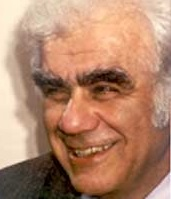
\includegraphics[width=2.5cm]{vlaa.jpg}
			};
		};
		
		\vspace{0.45cm}
		
		\begin{block}{\vspace*{-3ex}}
			Distance between \emph{kitten} and \emph{sitting} is $3$:
			\begin{itemize}
				\item kitten $\rightarrow$ sitten (substitution of ``s'' for ``k'')
				\item sitten $\rightarrow$ sittin (substitution of ``i'' for ``e'')
				\item sittin $\rightarrow$ sitting (insertion of ``g'' at the end)
			\end{itemize}
		\end{block}
	\end{frame}

	
	\begin{frame}
	    \begin{alertblock}{\textbf{The Approach:}}
	    \begin{itemize}
	        \item Compare test/training search queries with Levenshtein.
	        \item Use relevance of closest search query.
	    \end{itemize}
	    \end{alertblock}
	    
	    \begin{alertblock}{\textbf{The Future:}}
	    \begin{itemize}
	        \item Include brand information.
	        \item Implement SVM/SVR (``Do some actual machine learning'').
	    \end{itemize}
	    \end{alertblock}

       \begin{alertblock}{\textbf{The Problem:}}
	    \begin{itemize}
	        \item Lots of messy data (typos, inconsitency, etc).
	        \item SVM/SVR requires numbers.
	    \end{itemize}
	    \end{alertblock}
	    
	    \vspace{-0.3cm}
	    
	    \begin{alertblock}{\vspace*{-3ex}}
	    	\textbf{\textcolor{reddy}{Current rank on Kaggle:}} 1464
	    \end{alertblock}
	    
	\end{frame}
	
	\end{document}	